\documentclass{article}
\usepackage[utf8]{inputenc}
\usepackage[polish]{babel} 
\usepackage{graphicx}
\usepackage{float}
\usepackage{amsmath} 
\usepackage{hyperref}
\graphicspath{ {./images/} } 

\title{
    SPRAWOZDANIE \\ [0.6em]
    \large Metody Modelowania Matematycznego \\ [0.5em]
    \large Projekt nr 10
}

\author{Autorzy: Stanisław Oryl, Tomasz Kupski}
\date{\today}

\begin{document}

\maketitle

\section{Wprowadzenie}
Dany jest układ RLC, gdzie R, L, C to parametry modelu. \\
Należy zaimplementować symulator tego układu, umożliwiając uzyskanie odpowiedzi czasowych układu na pobudzenie przynajmniej trzema rodzajami sygnałów wejściowych. \\
Należy wykreślić charakterystyki częstotliwościowe Bodego (amplitudową i fazową) oraz odpowiedź układu.

\begin{figure}[H]
    \centering
    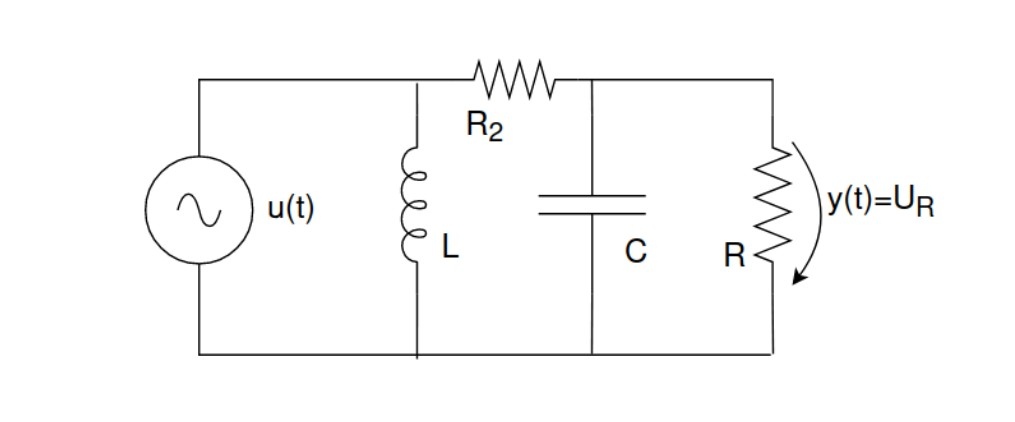
\includegraphics[width=0.8\textwidth]{Uklad.jpg}
    \caption{Zadany układ RLC.}
    \label{fig:uklad_rlc}
\end{figure}

\section{Część matematyczna}
Wyprowadzenie równań układu:

\begin{figure}[H]
    \centering
    \includegraphics[width=0.8\textwidth]{Matemattka.jpg}
    \caption{}
    \label{fig:matematyka}
\end{figure}

\section{Metoda symulacji}
Do wyznaczenia odpowiedzi czasowej układu wykorzystano jawną metodę Eulera, opierającą się na geometrycznej interpretacji równania różniczkowego. 
W każdym kroku symulacji $k$ w pierwszej kolejności wyznaczane są wartości prądu wejściowego $i_{\text{wej}}[k]$ oraz wyjściowego $i_{\text{wyj}}[k]$ na podstawie aktualnego stanu napięć w układzie:
\begin{equation}
    i_{\text{wej}}[k] = \frac{u_{\text{wej}}[k] - u_c[k]}{R_2}, \qquad i_{\text{wyj}}[k] = \frac{u_c[k]}{R}
\end{equation}

Następnie wyliczana jest pochodna napięcia na kondensatorze, która wyznacza kierunek stycznej:
\begin{equation}
    \frac{\mathrm{d}u_c[k]}{\mathrm{d}t} = \frac{i_{\text{wej}}[k] - i_{\text{wyj}}[k]}{C}
\end{equation}

Wzdłuż wyznaczonej stycznej obliczana jest kolejna (przyszła) wartość napięcia dla kroku $k+1$, z uwzględnieniem kroku czasu $\Delta t$:
\begin{equation}
    u_c[k+1] = u_c[k] + \frac{\mathrm{d}u_c[k]}{\mathrm{d}t} \cdot \Delta t
\end{equation}

\begin{figure}[H]
    \centering
    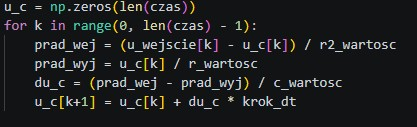
\includegraphics[width=0.8\textwidth]{met_euler.jpg}
    \caption{Metoda Eulera w kodzie}
    \label{fig:metoda_eulera}
\end{figure}

\section{Sygnały}
Generowane sygnały w programie:\\
-\textbf{Prostokątny} o określonym czasie trwania o zadanym okresie T , który po czasie 0.5 s zostaje wygaszony do zera.\\
-\textbf{Trójkątny}, o zadanej częstotliwości, rozpoczyna od zbocza narastającego.\\
-\textbf{Harmoniczny}, jest to funkcja sinus.\\




\begin{figure}[H]
    \centering
    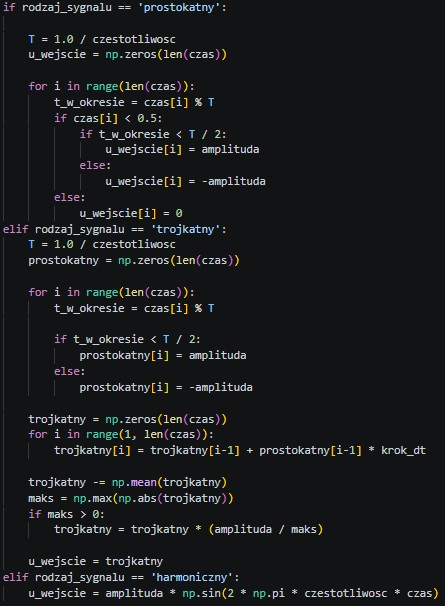
\includegraphics[width=0.8\textwidth]{sygnalyy.jpg}
    \caption{Rysunek przedstawia generowane sygnały w kodzie.}
    \label{fig:sygnalyy}
\end{figure}

\section{Symulacja}

\begin{figure}[H]
    \centering
    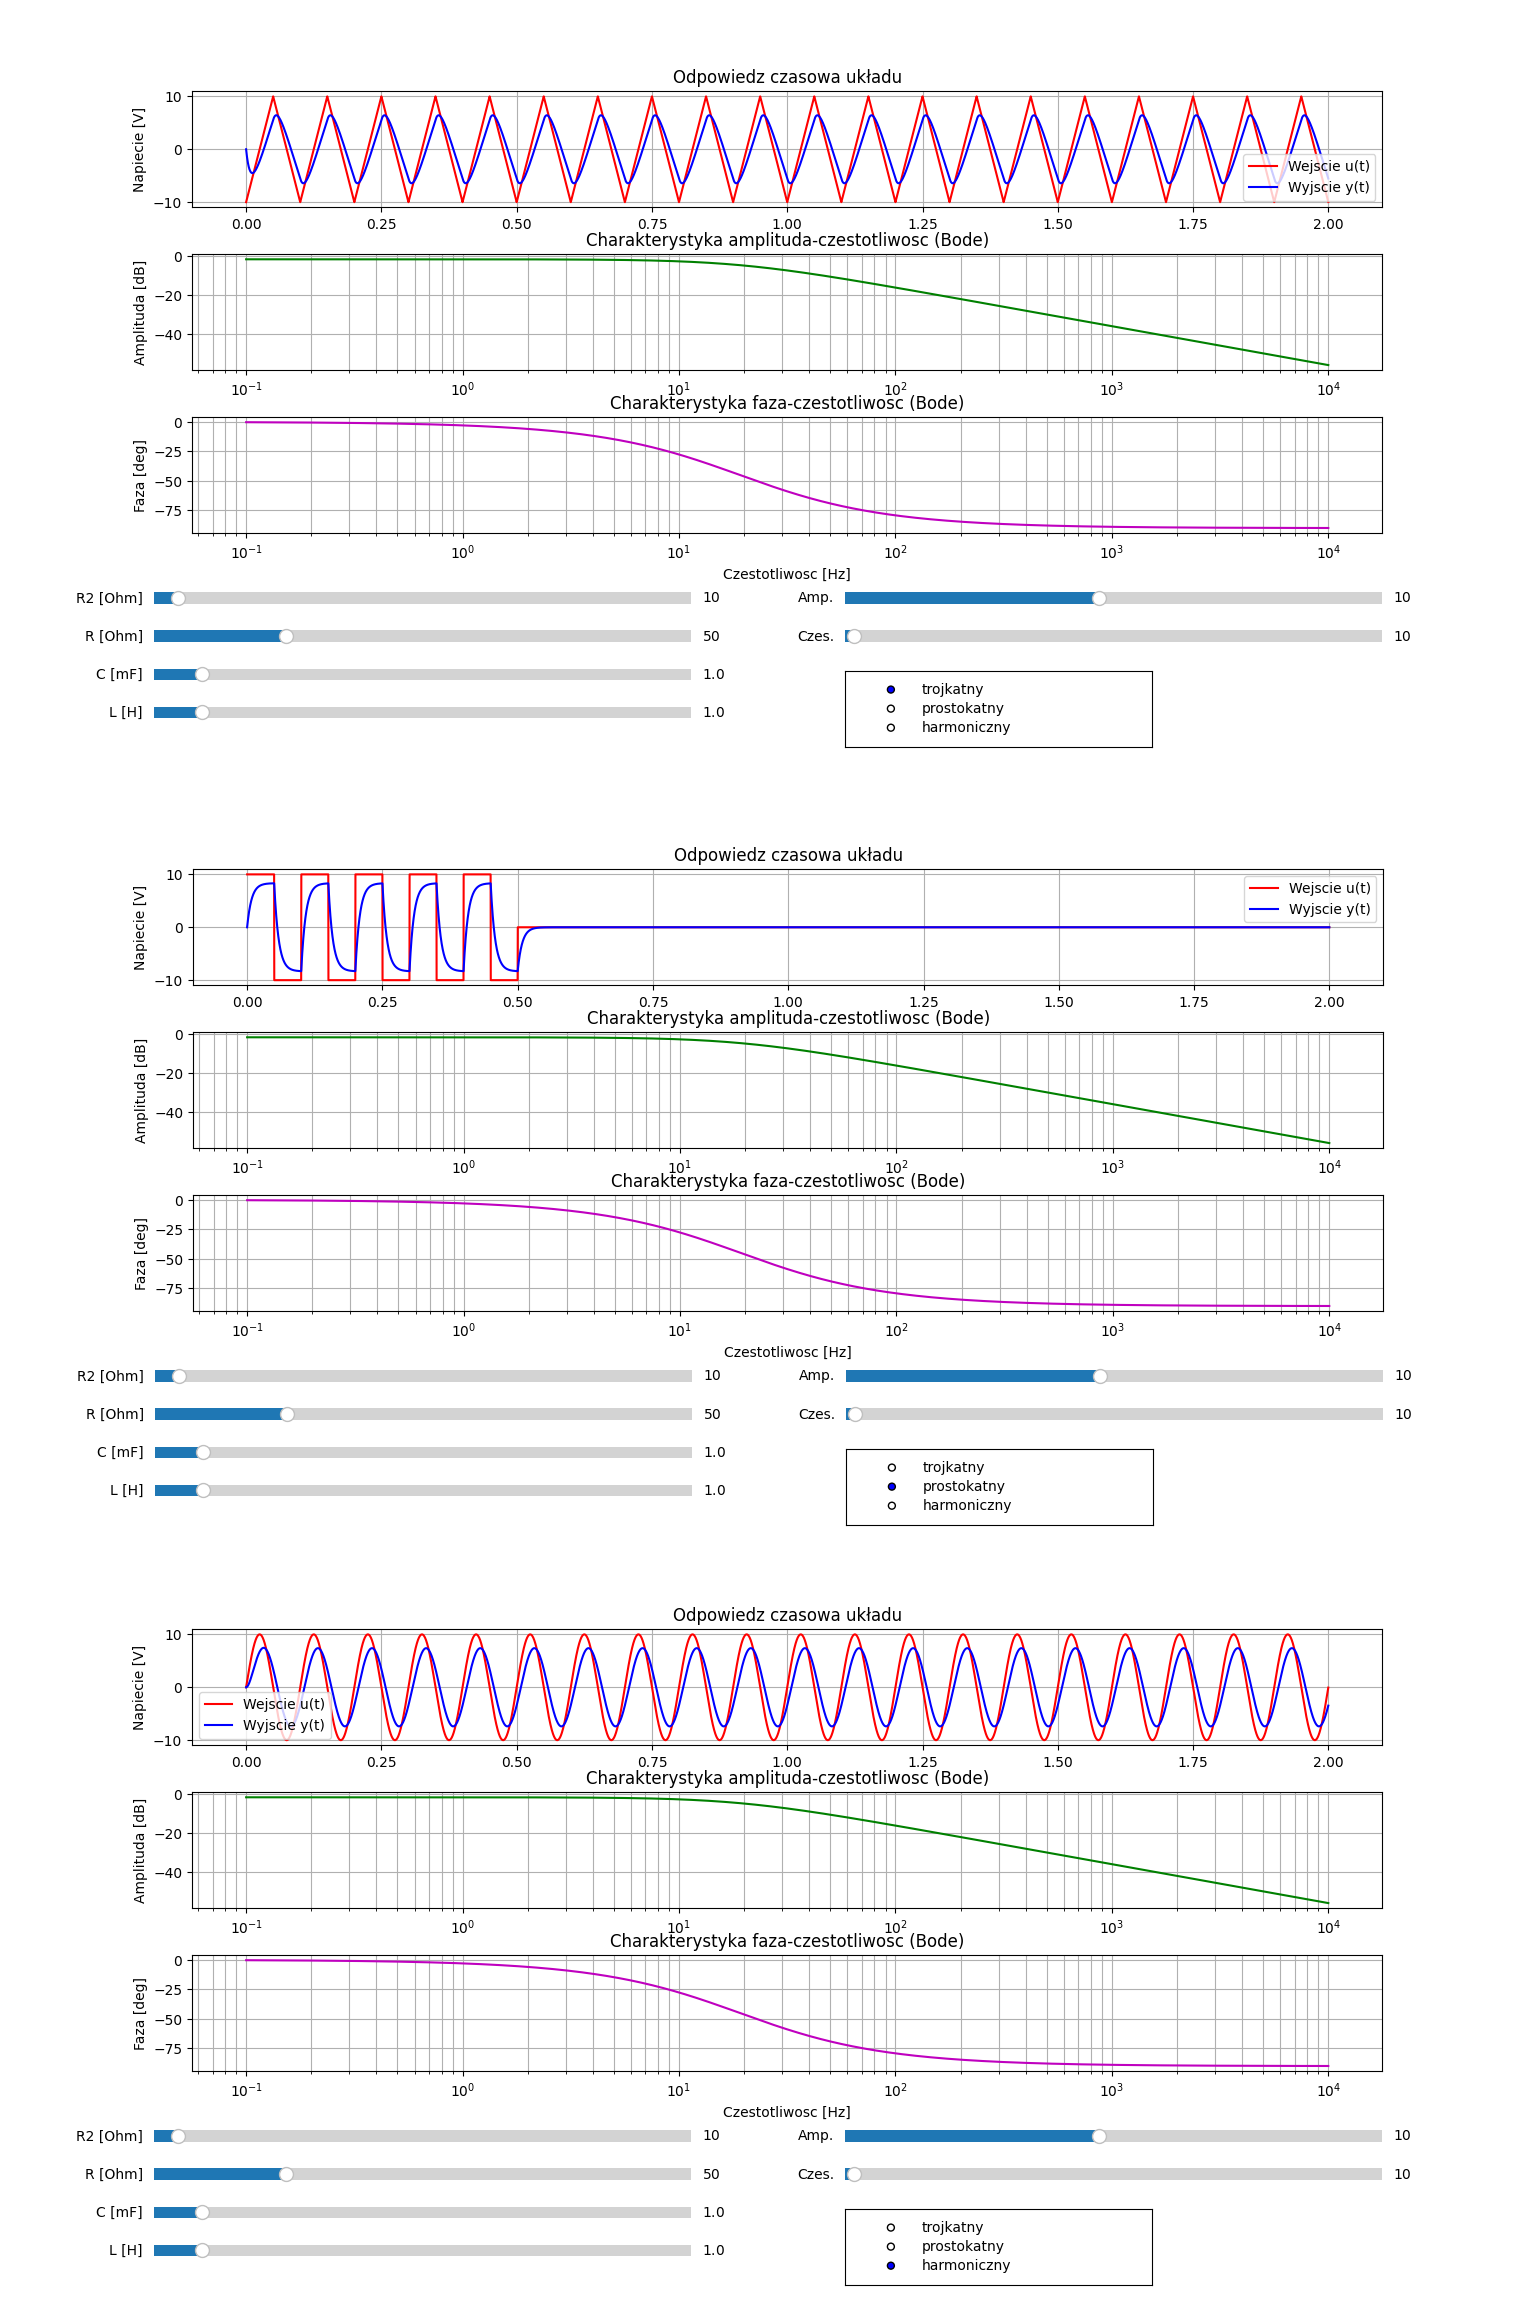
\includegraphics[width=0.8\textwidth]{obrazek_a.png}
    \caption{Rysunek przedstawia porównanie trzech sygnałów wejściowych (od góry: trójkątny, prostokątny o skończonym czasie trwania, harmoniczny sinusoidalny) oraz odpowiedzi układu na te sygnały.}
    \label{fig:obrazek_a}
\end{figure}

\begin{figure}[H]
    \centering
    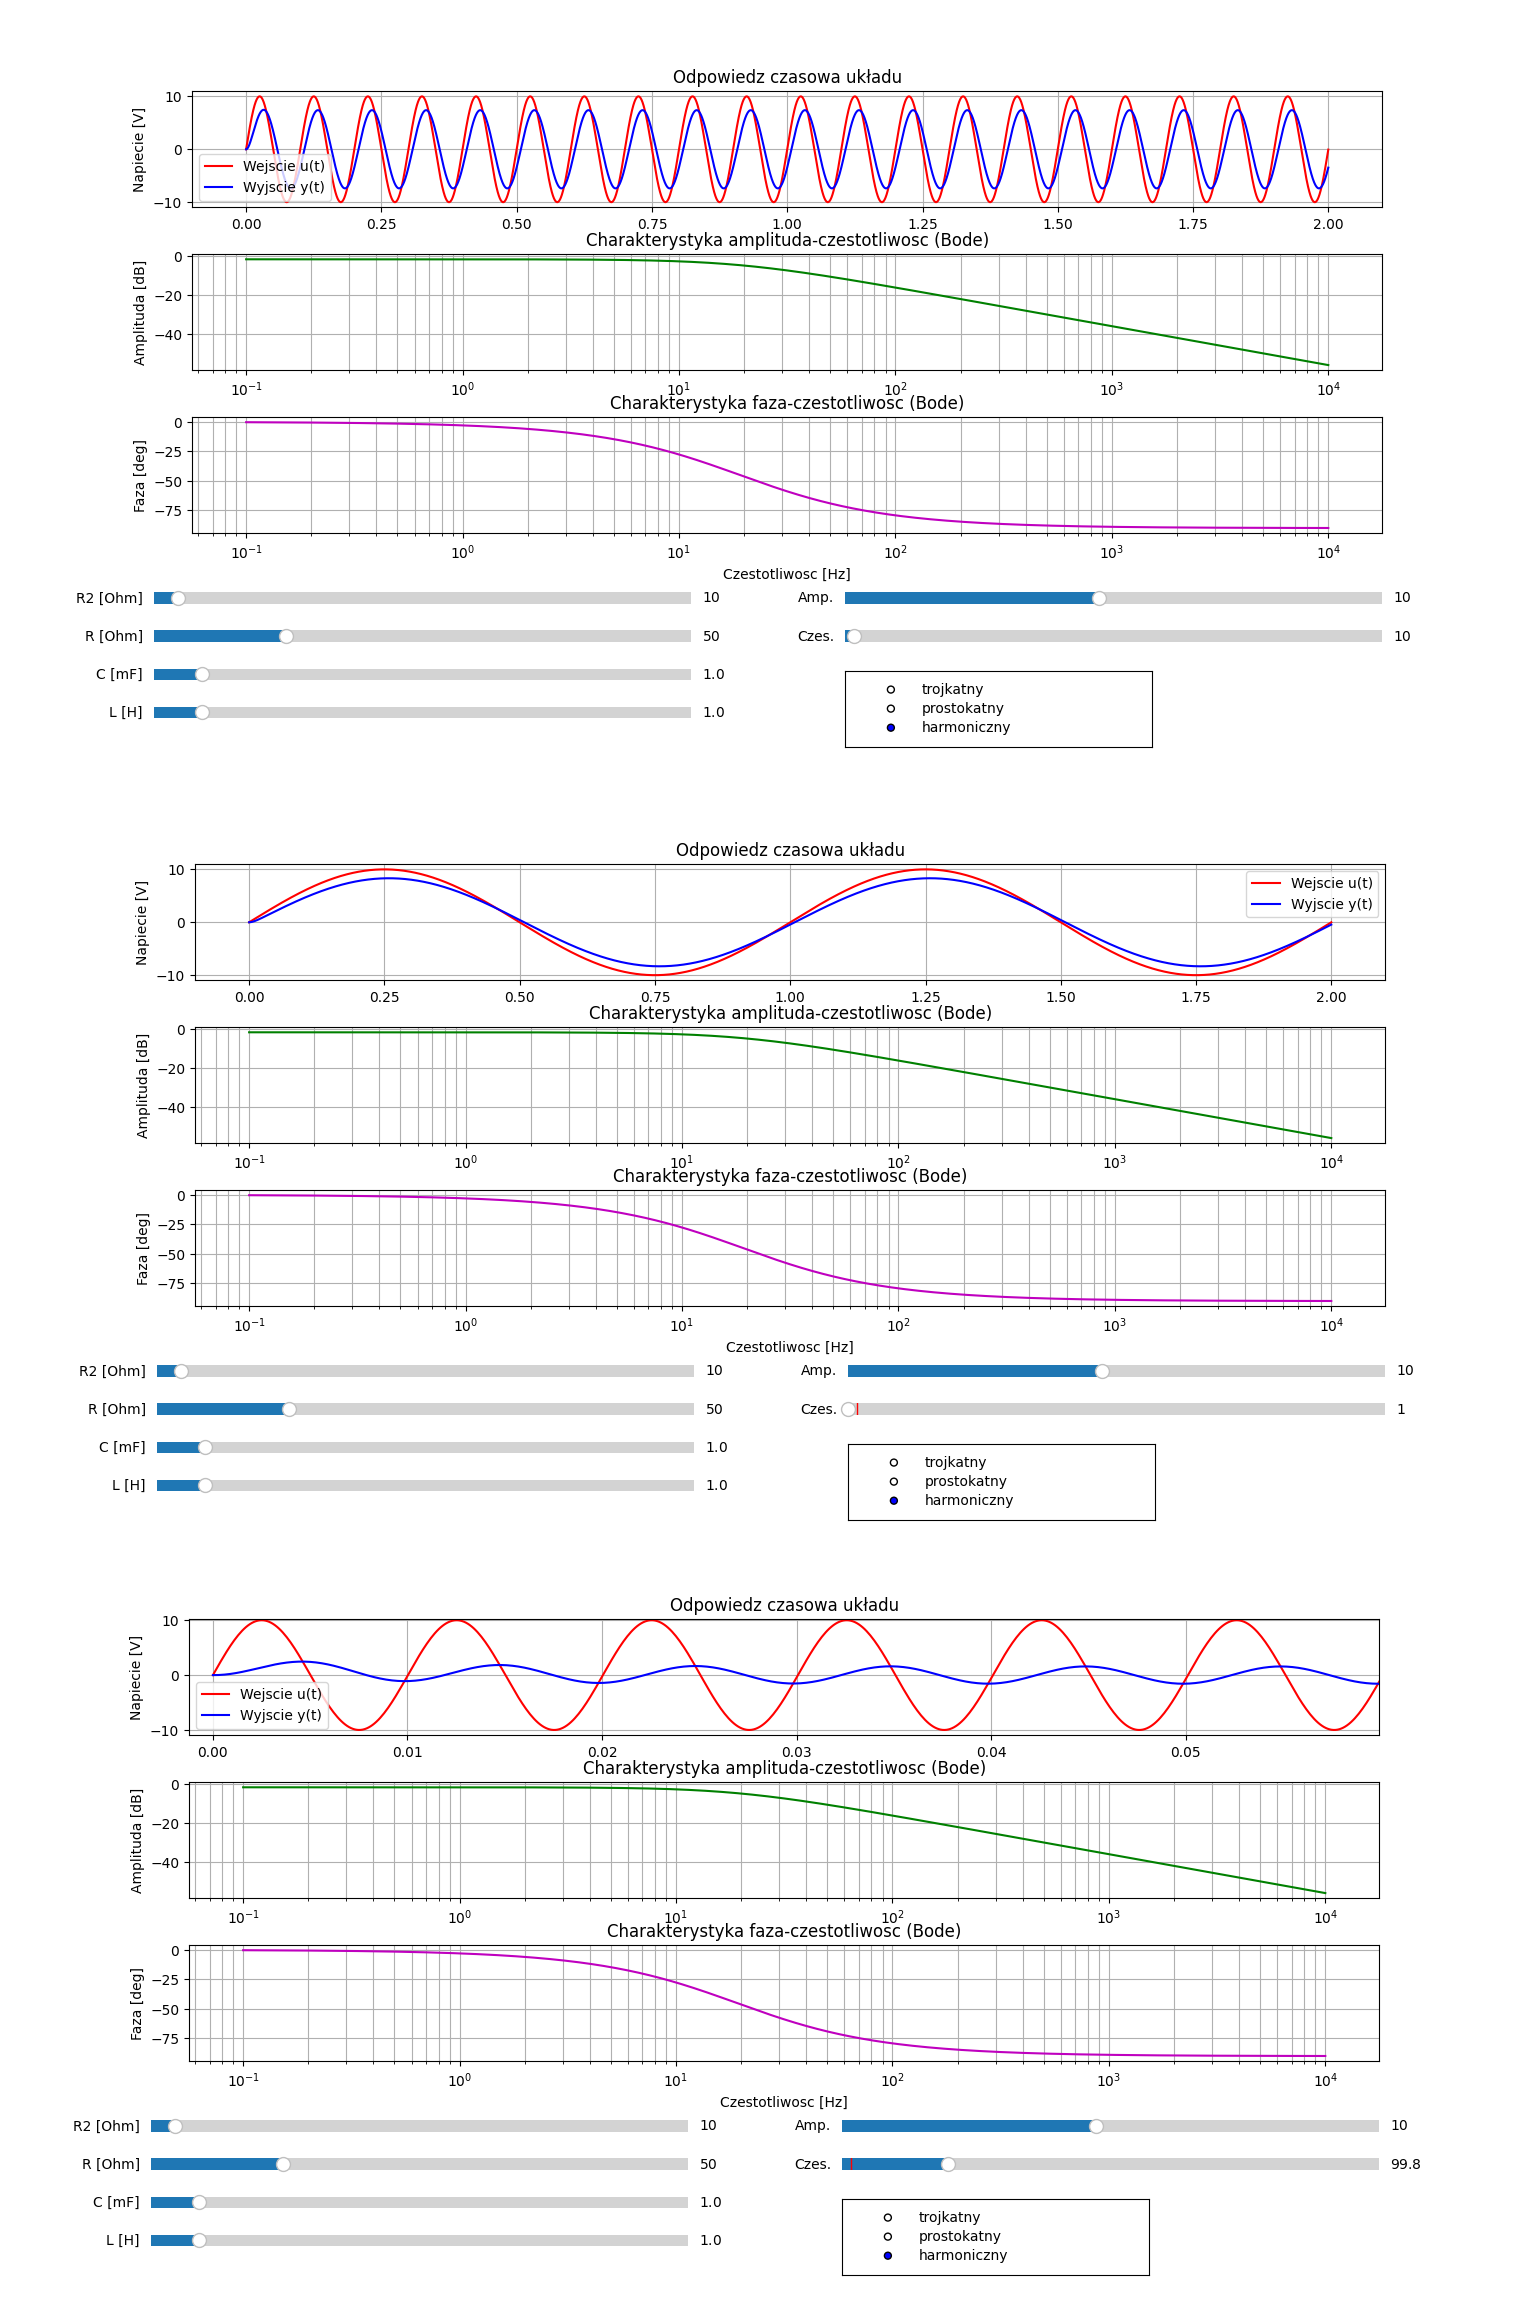
\includegraphics[width=0.8\textwidth]{obrazek_b.png}
    \caption{Rysunek przedstawia porównanie sygnałów wejściowych harmonicznych o trzech wartościach częstotliwości (od góry: 10Hz, 1Hz, ok. 100Hz - widok przybliżony). Na bazie tego porównania można zauważyć, iż charakterystyki Bodego pokrywają się z odpowiedziami układu na pobudzenia o różnych częstotliwościach.}
    \label{fig:obrazek_b}
\end{figure}

\begin{figure}[H]
    \centering
    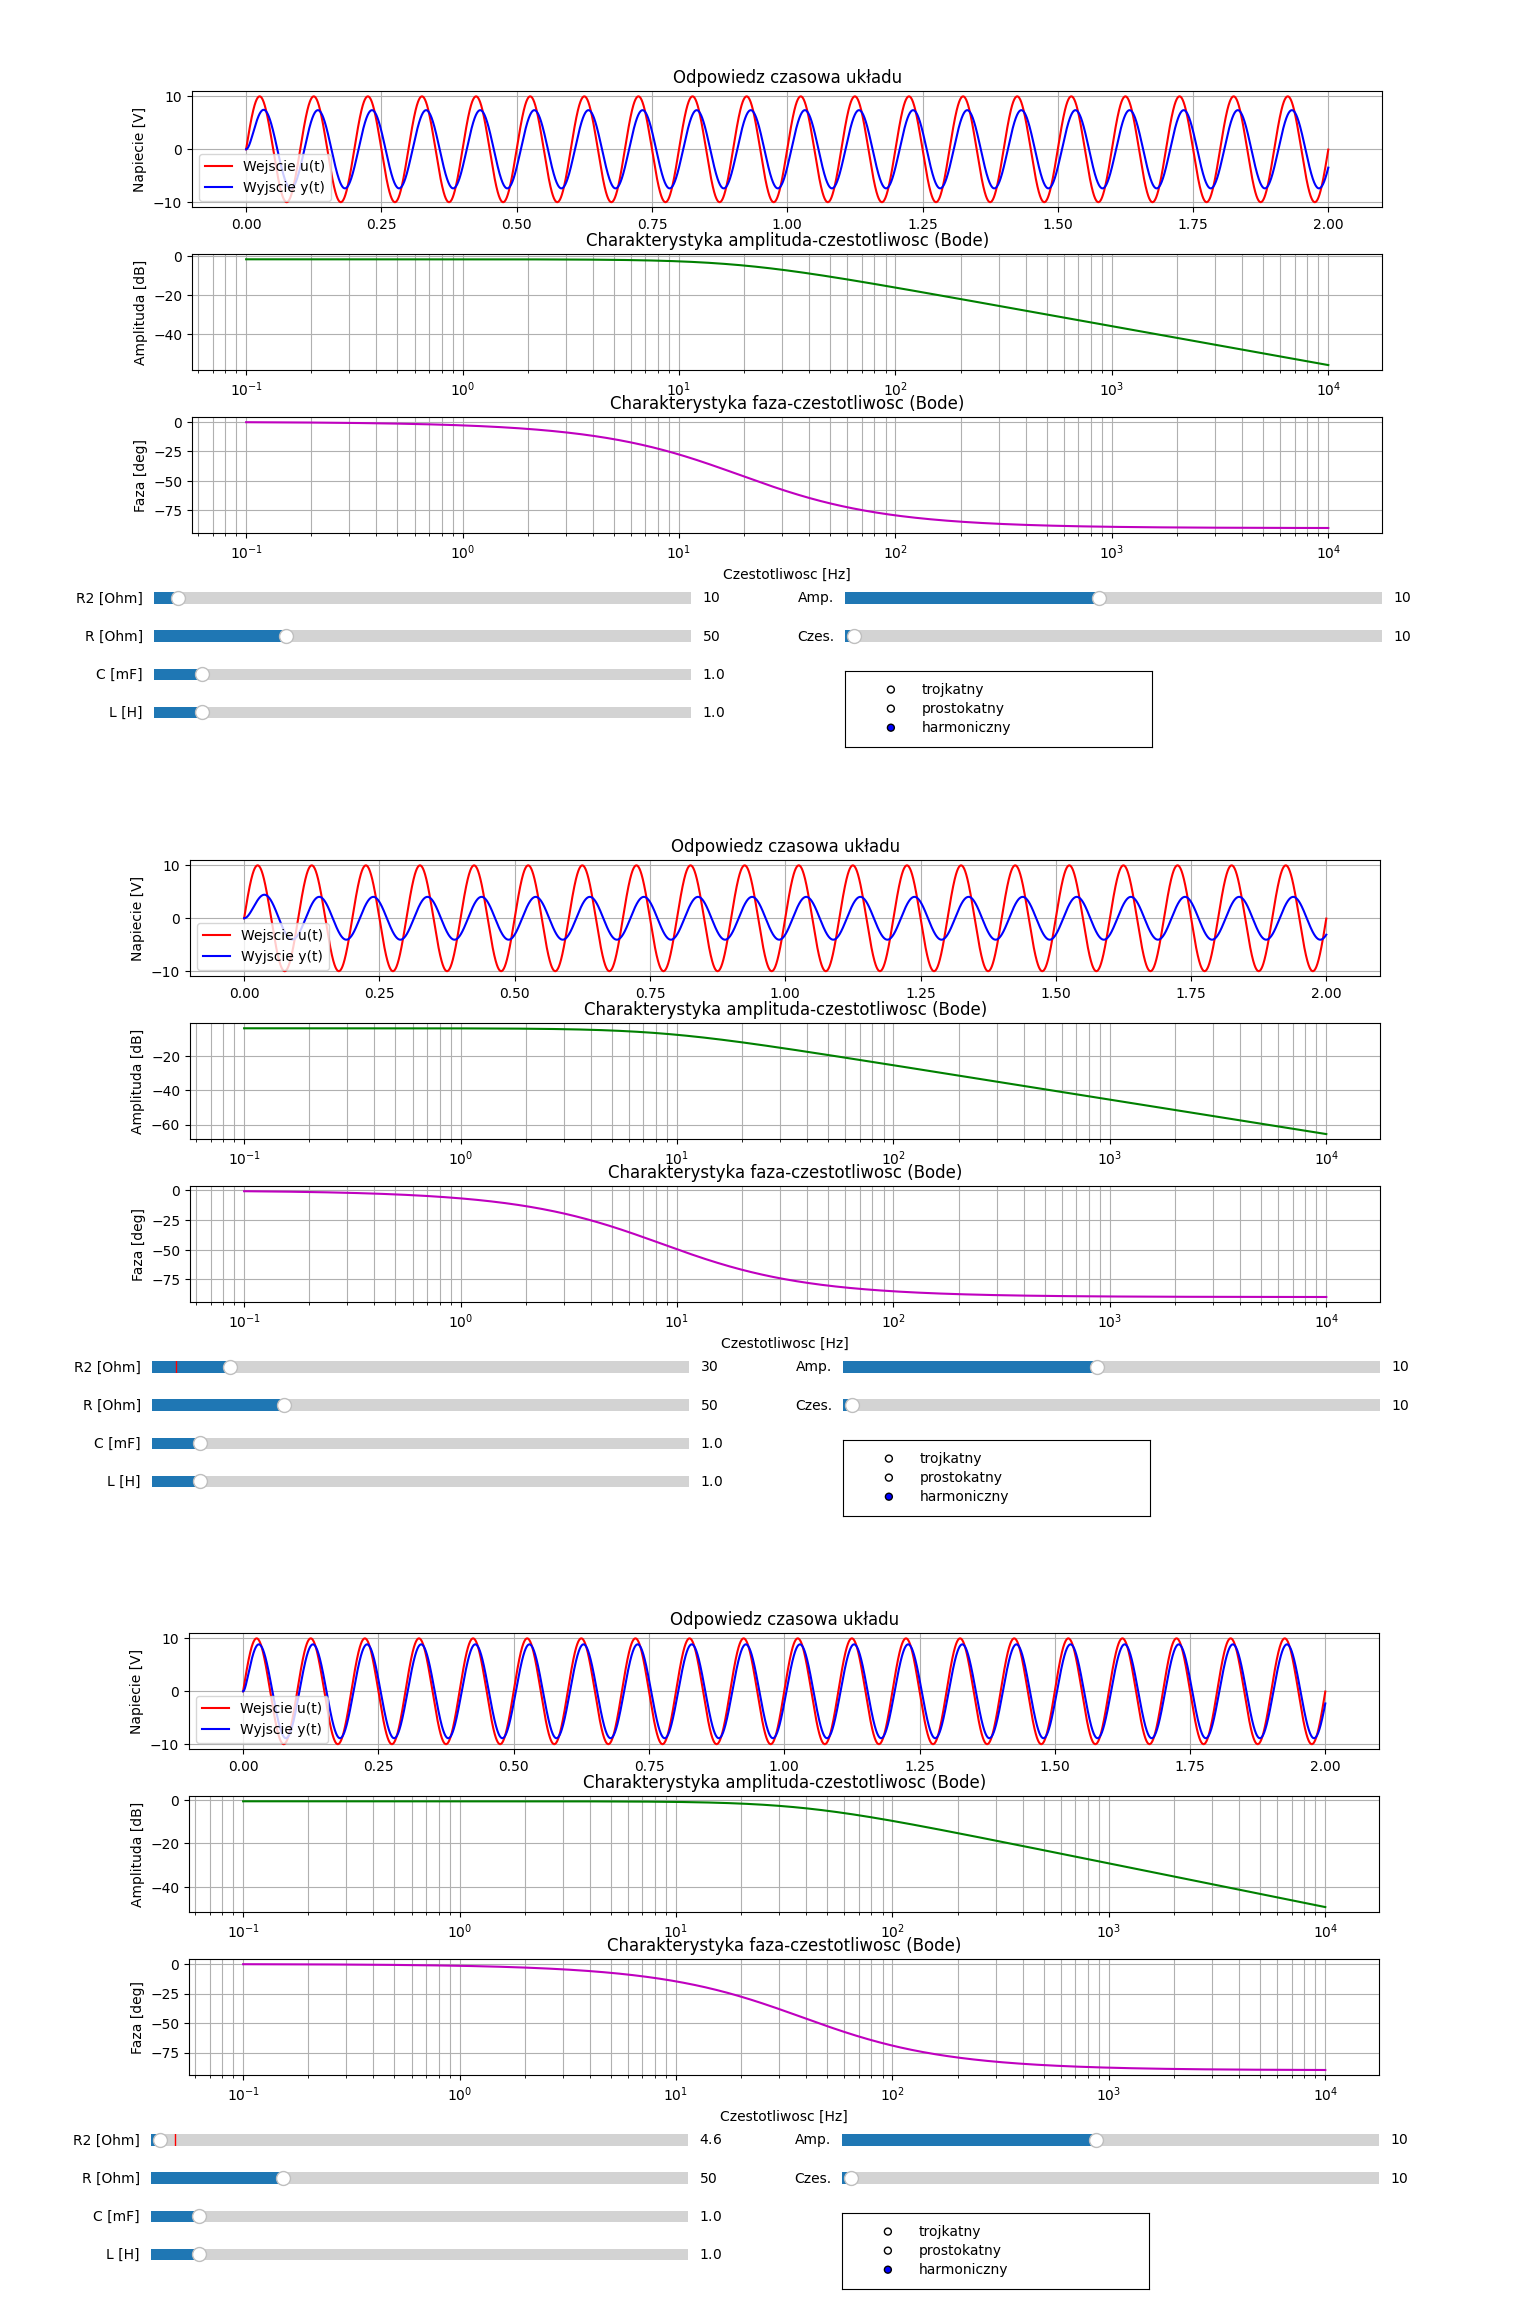
\includegraphics[width=0.8\textwidth]{obrazek_c.png}
    \caption{Rysunek przedstawia porównanie odpowiedzi układu oraz charakterystyk Bodego ze zmienionym parametrem $R_2$ układu.}
    \label{fig:obrazek_c}
\end{figure}

\begin{figure}[H]
    \centering
    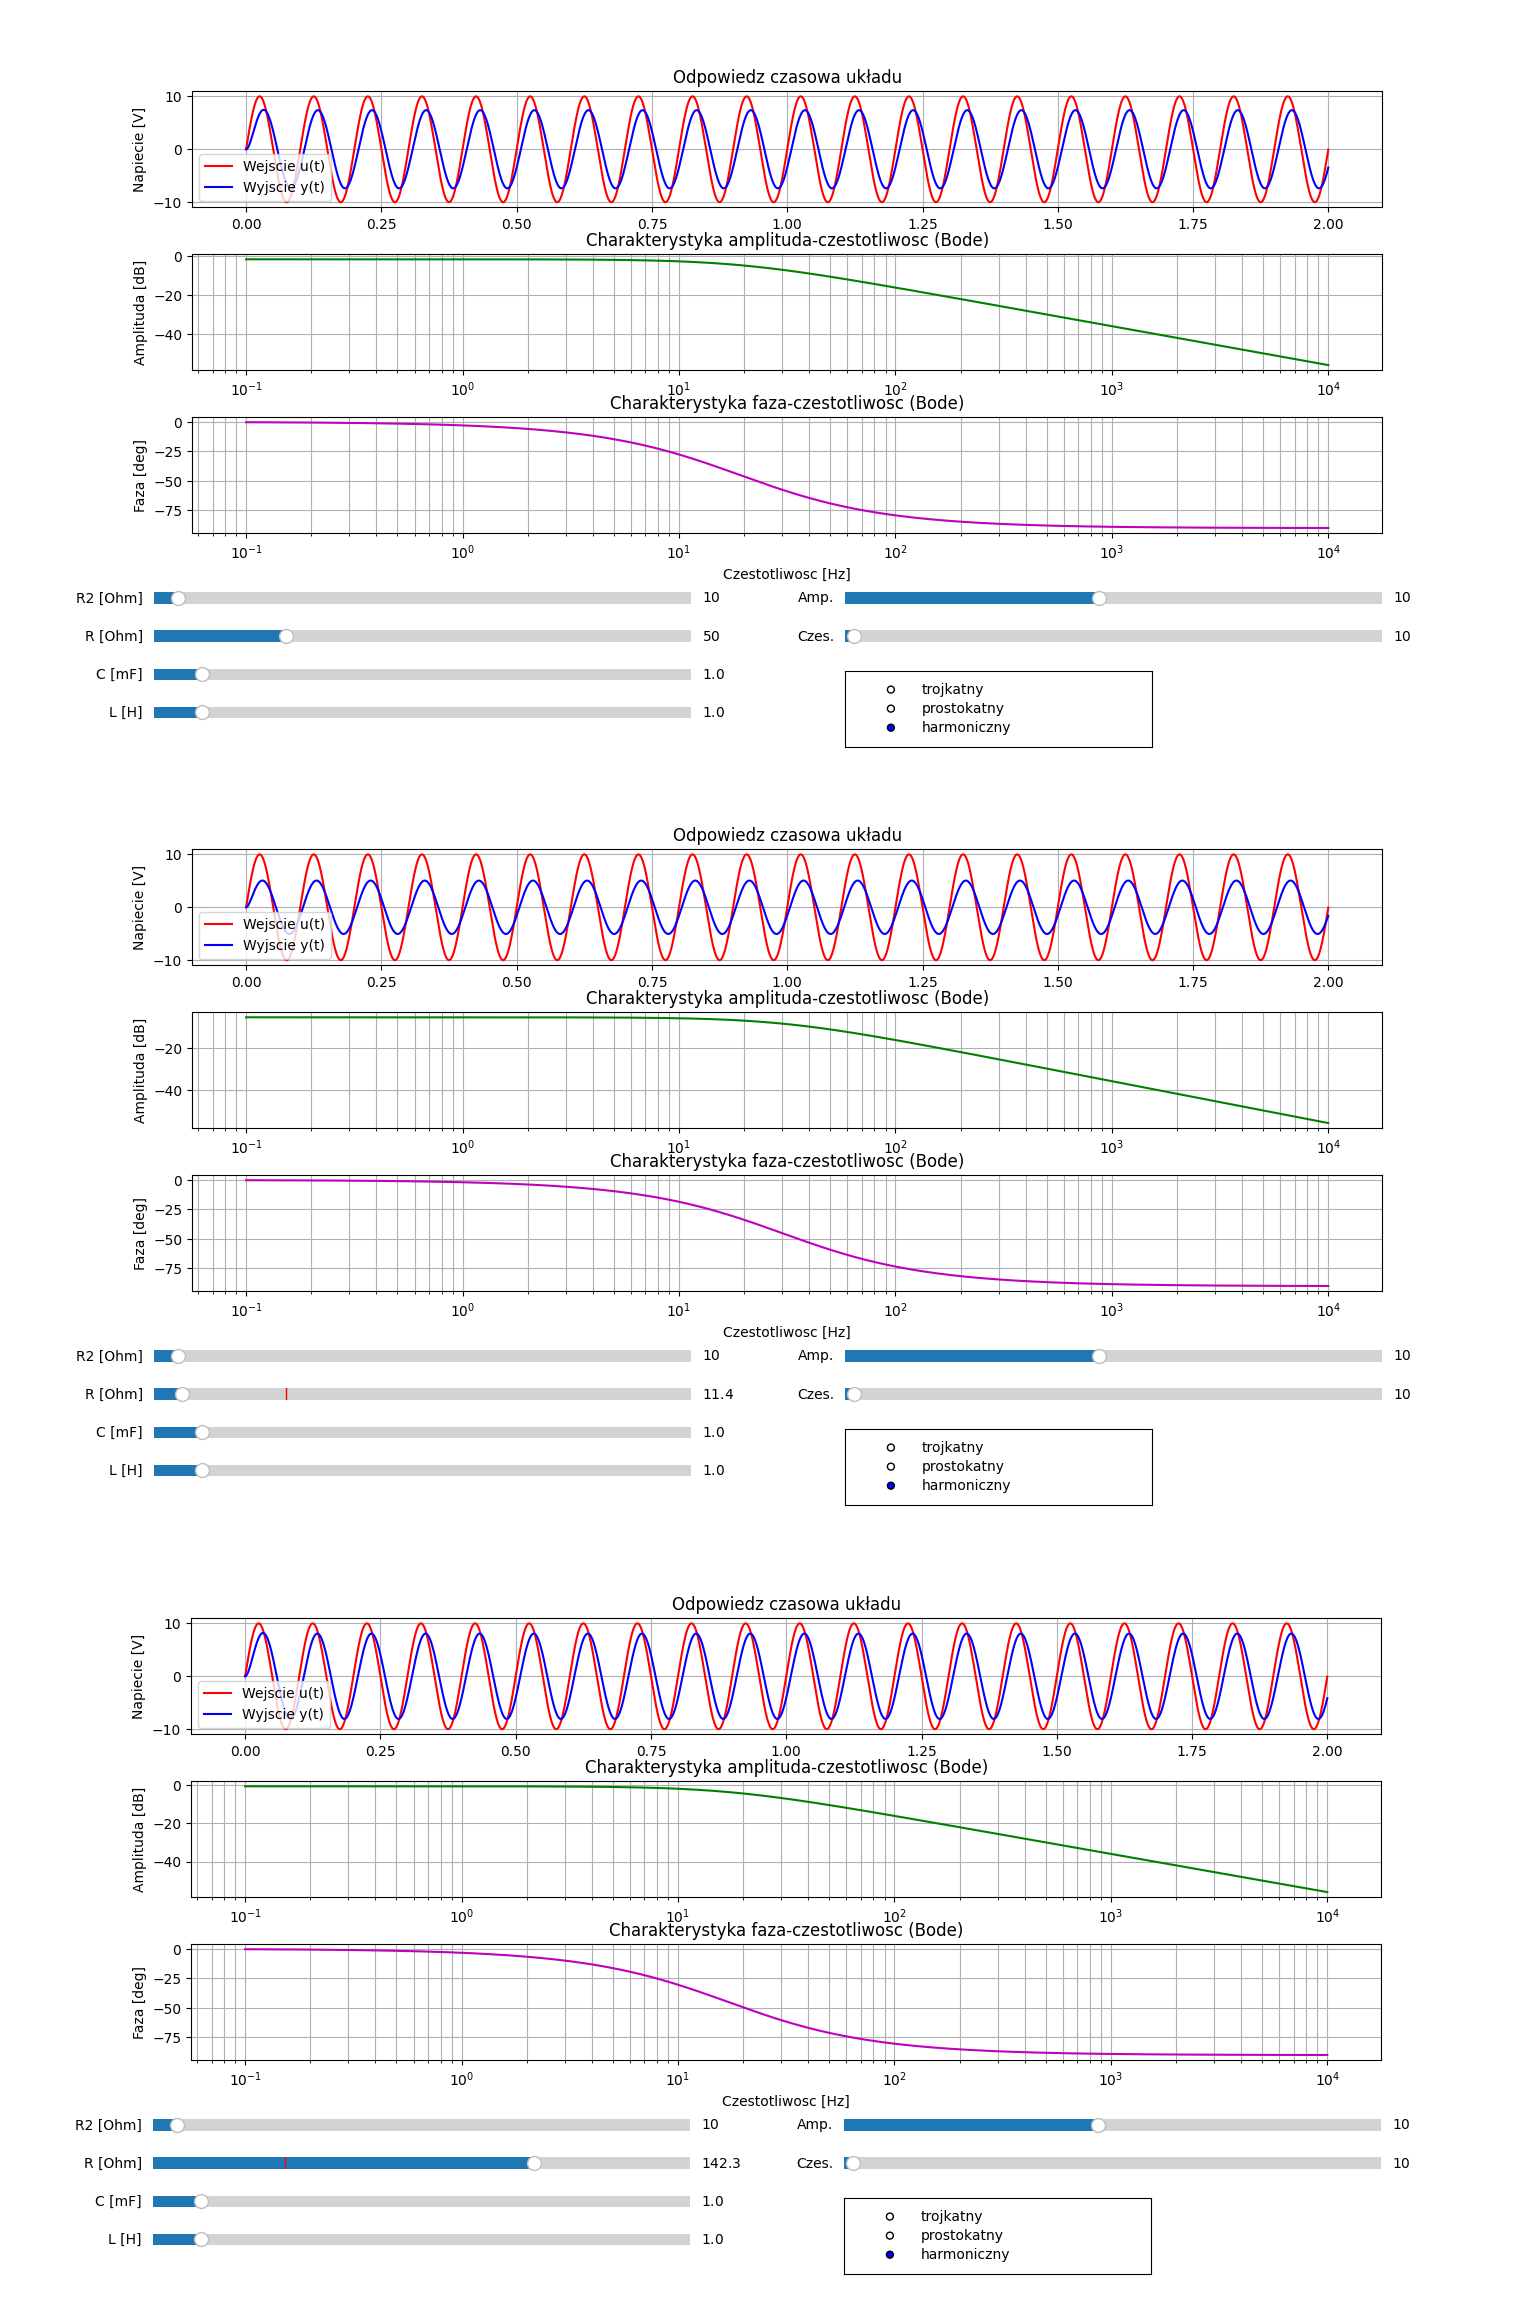
\includegraphics[width=0.8\textwidth]{obrazek_d.png}
    \caption{Rysunek przedstawia porównanie odpowiedzi układu oraz charakterystyk Bodego ze zmienionym parametrem $R$ układu.}
    \label{fig:obrazek_d}
\end{figure}

\begin{figure}[H]
    \centering
    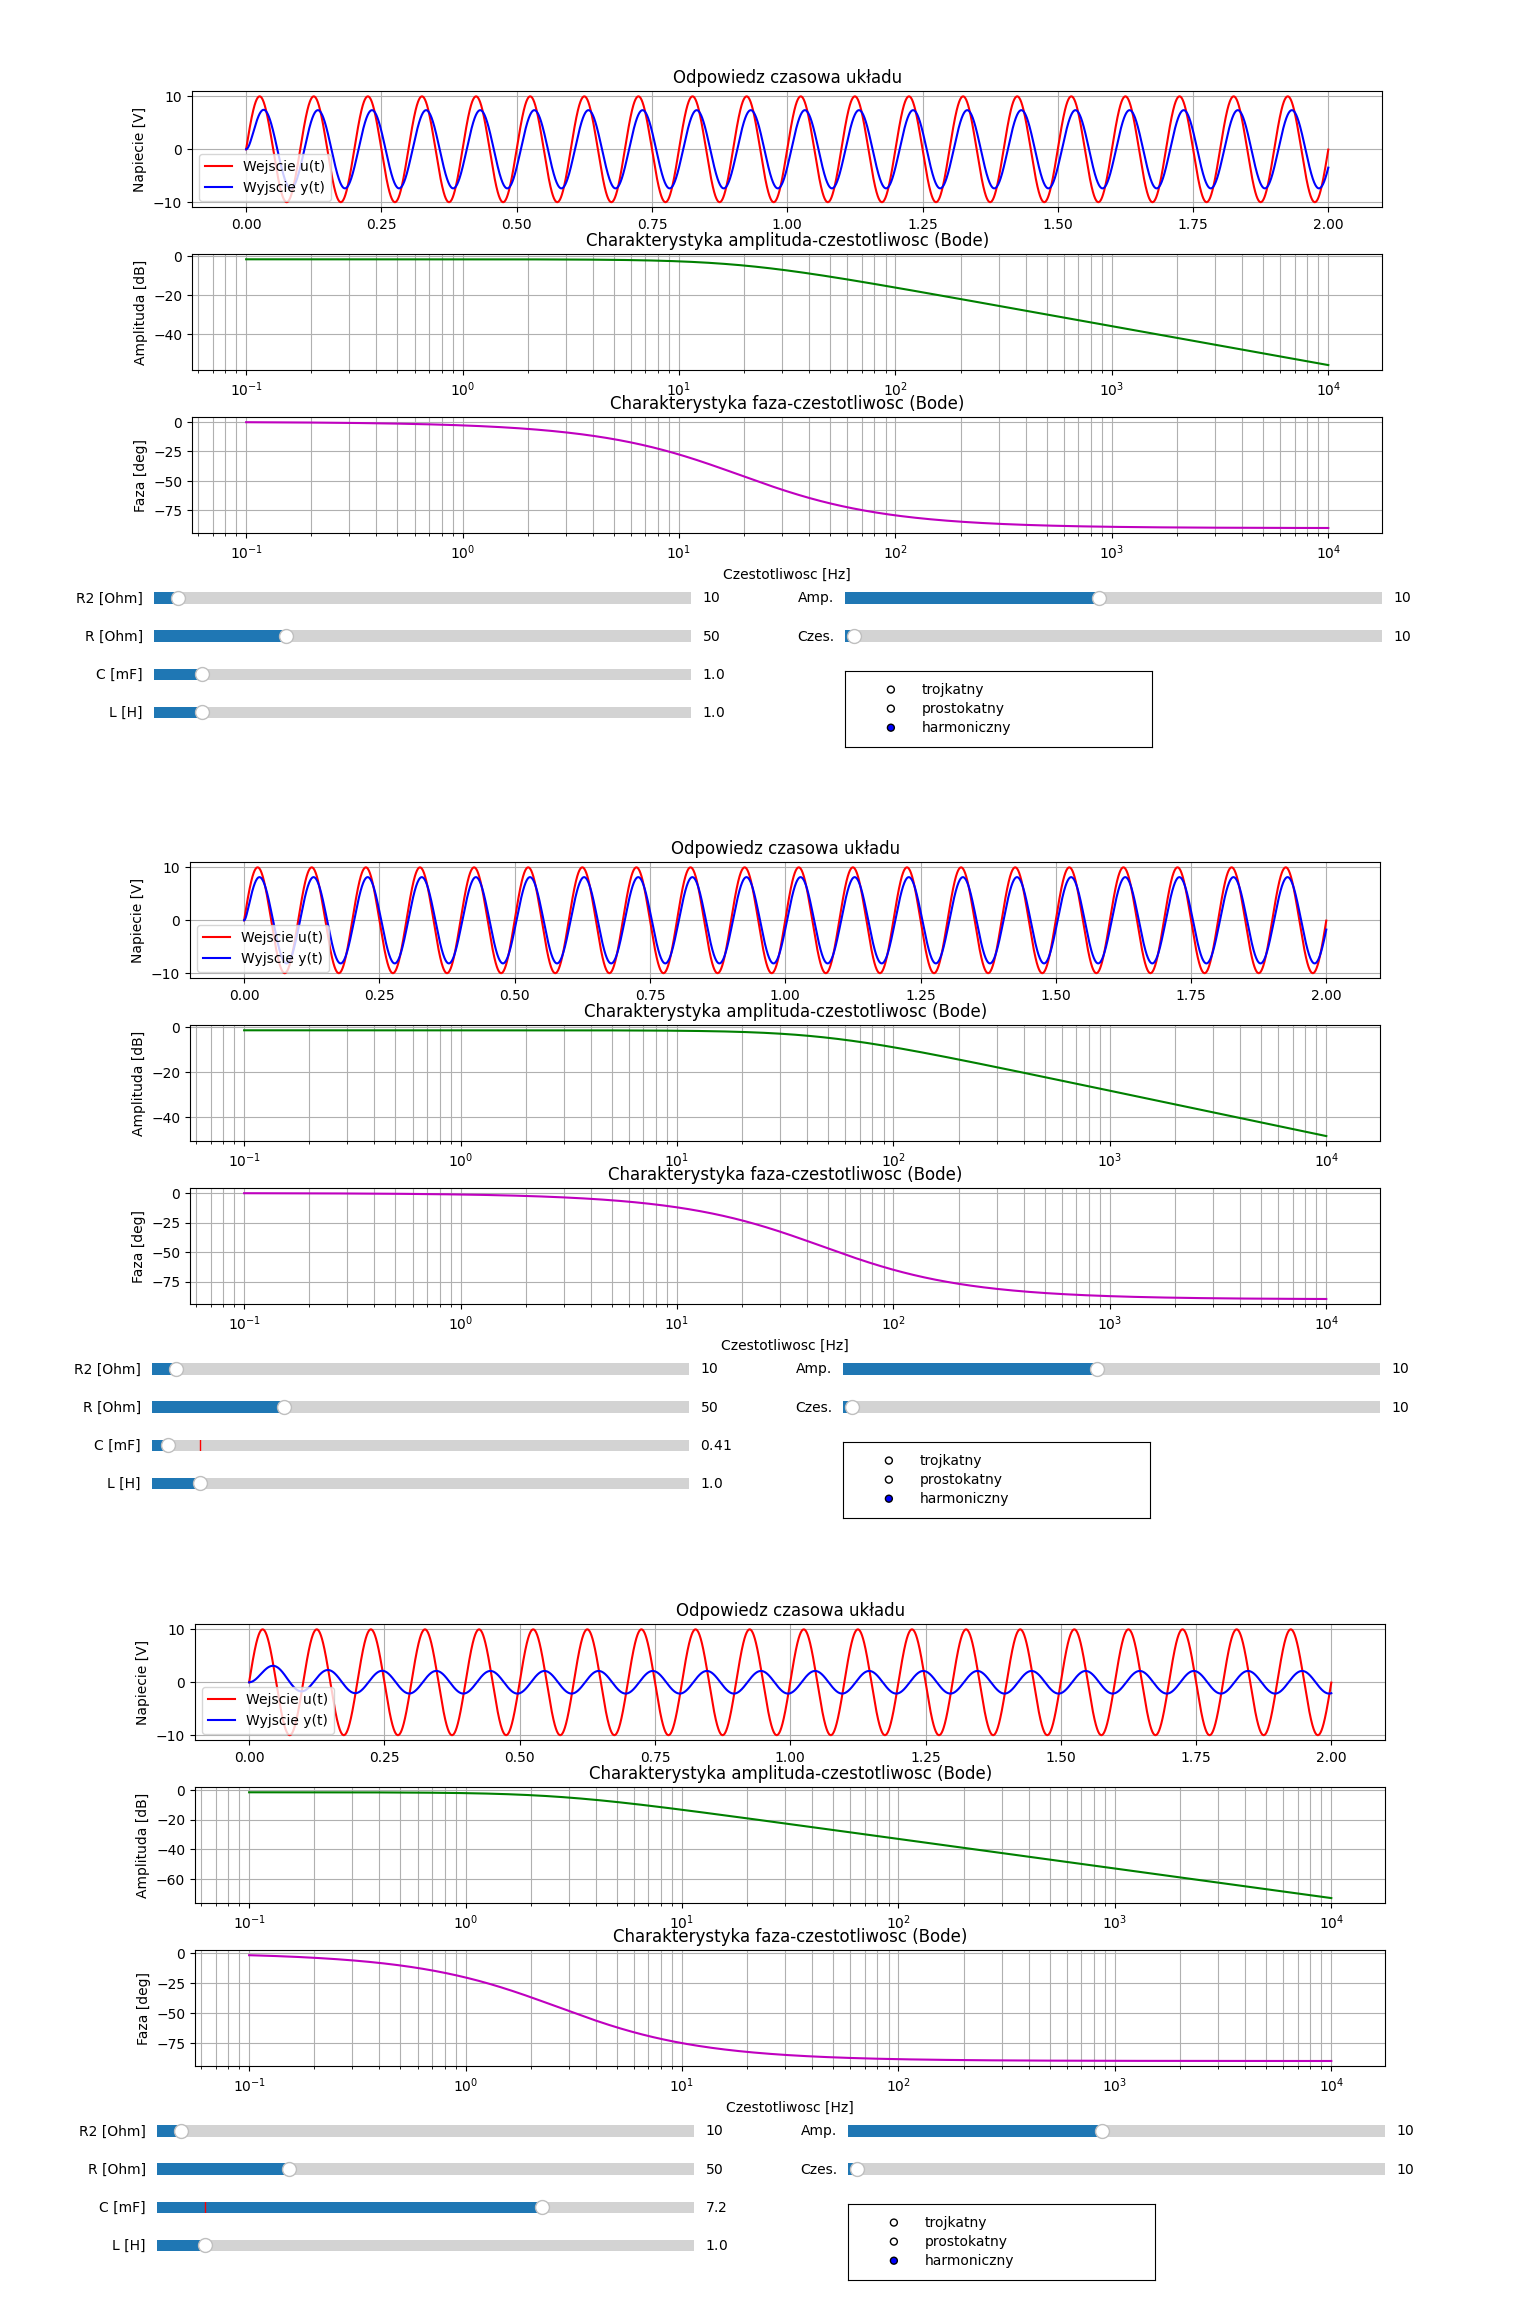
\includegraphics[width=0.8\textwidth]{obrazek_e.png}
    \caption{Rysunek przedstawia porównanie odpowiedzi układu oraz charakterystyk Bodego ze zmienionym parametrem $C$ układu.}
    \label{fig:obrazek_e}
\end{figure}

\begin{figure}[H]
    \centering
    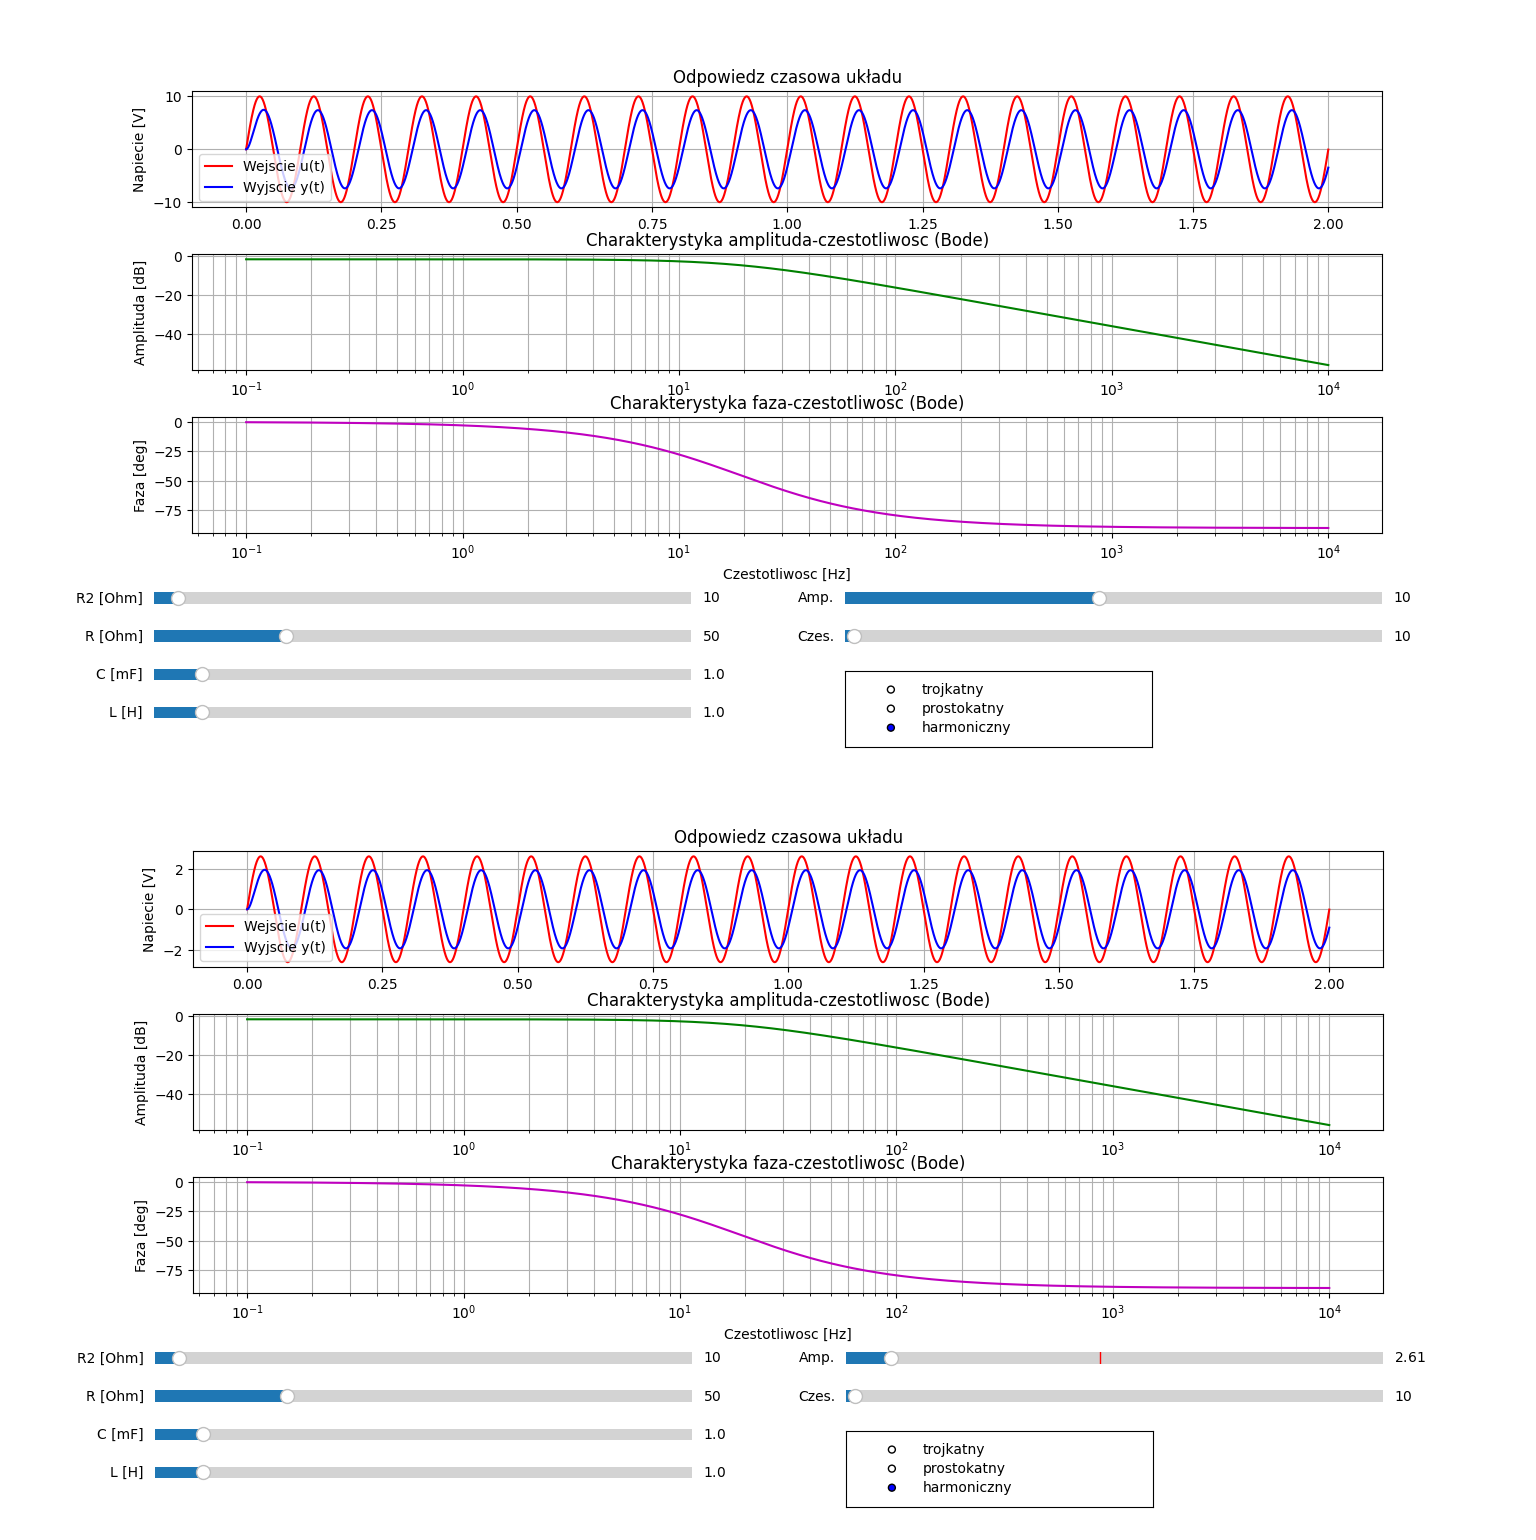
\includegraphics[width=0.8\textwidth]{obrazek_f.png}
    \caption{Rysunek przedstawia porównanie sygnałów wejściowych o różnych amplitudach. Wykres jest skalowany zależnie od amplitudy, lecz wartości na osi się zmieniają.}
    \label{fig:obrazek_f}
\end{figure}
\begin{figure}[H]
    \centering
    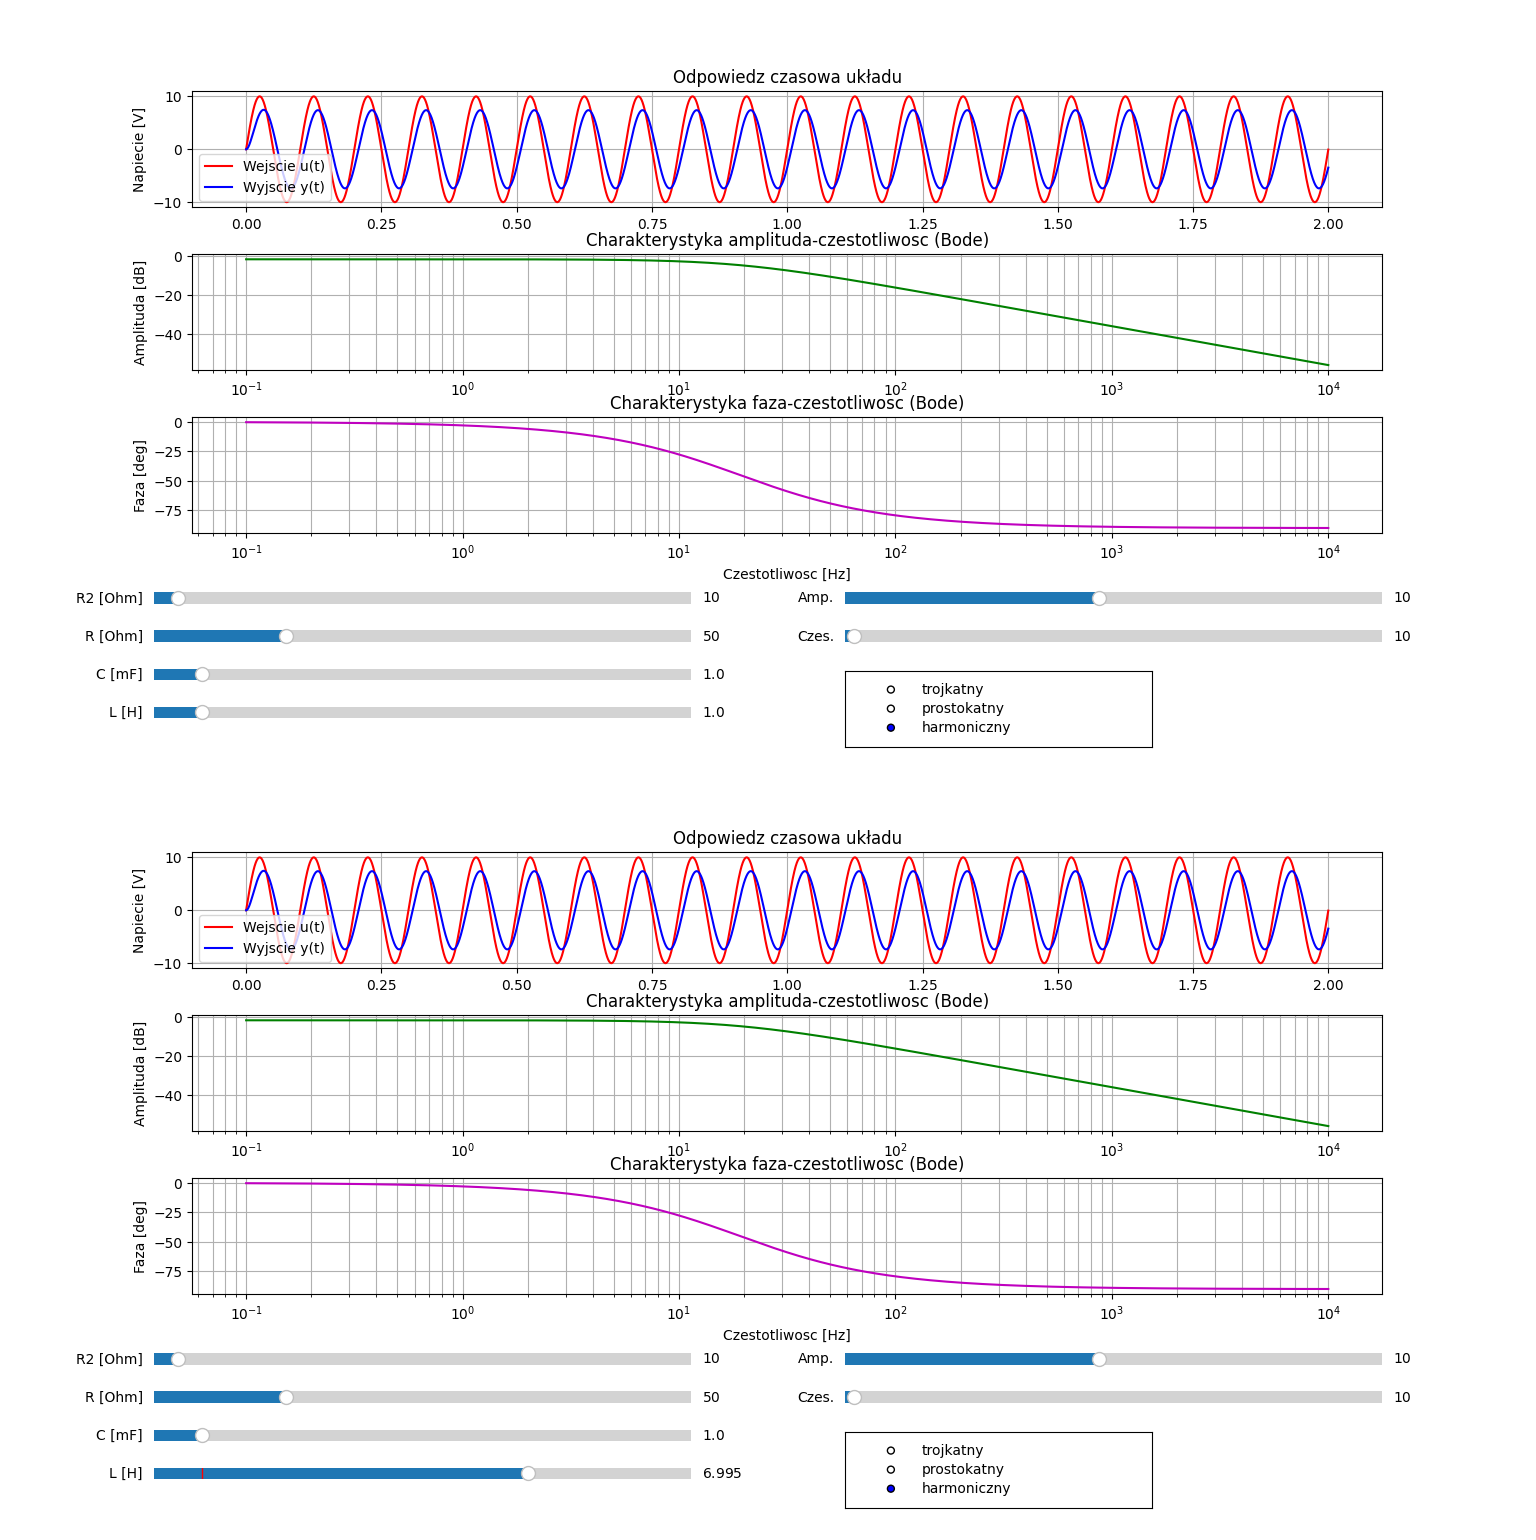
\includegraphics[width=0.8\textwidth]{obrazek_g.png}
    \caption{Rysunek przedstawia porównanie odpowiedzi układu roaz charakterystyk Bodego ze zmienionym parametrem $L$ układu. Zauważalne jest, iż zmiana wartości tego parametru nie wpływa na zachowanie układu}
    \label{fig:obrazek_g}
\end{figure}

\section{Wnioski}
Cewka L nie wpływa na transmitancję $\frac{U_R(s)}{U(s)}$, ponieważ jest połączona równoległe z idealnym źródłem napięcia. W programie symulacyjnym został umieszczony suwak do zmiany tej wartości, żeby zaprezentować, iż nie wpływa ona na odpowiedź układu ani charakterystyki Bodego. $\\$Układ zachowuje się jak układ I rzędu, czyli filtr dolnoprzepustowy. Potwierdza to kształt charakterystyk Bodego – spadek wzmocnienia o 20$\frac{dB}{dek}\ $ oraz przesunięcie fazowe $-90^\circ$. Znając działanie tego układu można wywnioskować, iż symulacja spełnia teoretyczne założenia. Zmiana wartości elementów układu (pomijając L) zmienia kształt odpowiedzi układu oraz charakterystyk Bodego. Wraz ze wzrostem częstotliwości sygnału zauważalne na wykresie odpowiedzi układu są właściwości odczytywane z charakterystyk Bodego – spadek wzmocnienia oraz przesunięcie fazowe.$\\$Ze względu na prostotę układu (I rząd) do symulacji działania kondensatora wykorzystano metodę Eulera, która okazała się być wystarczająco dokładna dla tej symulacji. Rozważane było również użycie algorytmu Rungego-Kutty, lecz zmiana dokładności nie była zauważalna gołym okiem.

\section{Źródła}
\begin{itemize} 

\item wiedza oraz materiały z przedmiotów Obwody i Sygnały, Podstawy Automatyki oraz Zasady Optymalizacji w Automatyce 

\item \url{https://pl.wikipedia.org/wiki/Metoda_Eulera} 

\item \url{https://pl.wikipedia.org/wiki/Algorytm_Rungego-Kutty} 

\item dokumentacja biblioteki Matplotlib 

\end{itemize} 

\end{document}